%
% $Id: piano_z.tex 14 2014-02-04 22:36:30Z nicb $
%
\svnInfo $Id: piano_z.tex 14 2014-02-04 22:36:30Z nicb $

\section{Il piano Z\label{sec:pianoz}}

La rappresentazione delle caratteristiche della funzione di trasferimento di
un filtro sul \emph{piano z} complesso permette di capirne meglio il
funzionamento.

Riprendiamo il nostro filtro semplice

\begin{equation}\label{eq:simple fir}
	y_t = x_t - a_1 x_{t-1}
\end{equation}

Se sostituiamo in \ref{eq:simple fir} $x_t$ con un fasore, l'effetto di questo
filtro equivale alla moltiplicazione dell'ingresso per la funzione complessa

\begin{equation}\label{eq:simple transf function}
	1 - a_1 e^{-i \omega} = 1 - a_1 z^{-1}
\end{equation}

perch\'e abbiamo introdotto la stenografia $z = e^{i \omega}$.

Abbiamo quindi una funzione di trasferimento complessa  $\mathpzc{H} ( z )$
alla quale corrisponde la risposta in frequenza

\begin{equation}\label{eq: complex freq response}
		H ( \omega ) = \mathpzc{H} ( e^{i \omega} )
\end{equation}

In sostanza, la risposta in frequenza \`e la funzione di trasferimento della
variabile complessa $z$ \emph{valutata sul cerchio unitario}.
I valori di $\omega$ che ci interessano vanno da $\omega = 0$ alla frequenza
di Nyquist $\omega = \pi$ radianti per campione. Si tratta quindi della met\`a
superiore del cerchio nel piano $z$, come illustrato in Fig.\vref{fig: z plane frequency axis}
\begin{figure}[htp]
\begin{center}
	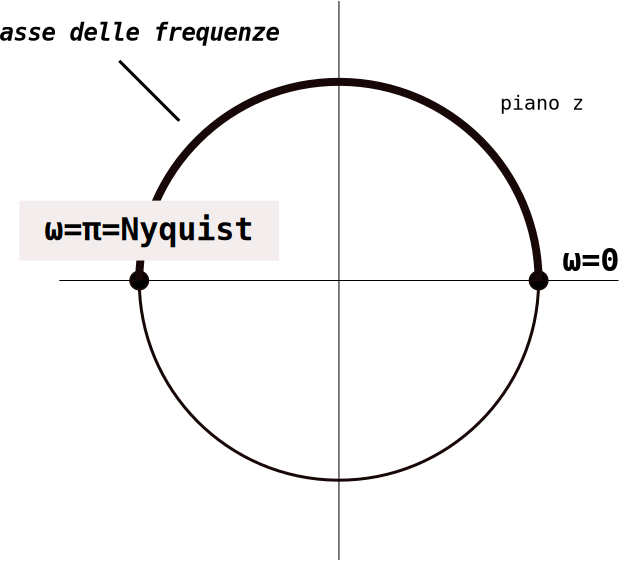
\includegraphics[width=0.4\textwidth]{\imagedir/frequency_axis_z_plane}
	\caption{L'asse delle frequenze sul piano $z$.\label{fig: z plane frequency axis}}
\end{center}
\end{figure}

Ora guardiamo pi\`u attentamente la funzione di trasferimento del nostro
esempio. Essa \`e

\begin{equation}\label{eq: simple transfer function 2}
				\mathpzc{H} ( z ) = 1 - a_1 z^{-1}
\end{equation}

Riscriviamola ora come rapporto di polinomi moltiplicando sopra e sotto per $z$:

\begin{equation}\label{eq: simple transfer function 3}
				\mathpzc{H} ( z ) = 1 - a_1 z^{-1} = \frac{z}{z} - \frac{a_1}{z} = \frac{z - a_1}{z}
\end{equation}

In questo modo appaiono chiaramente le radici dell'equazione:
c'\`e uno zero nel numeratore a $z = a_1$ e uno zero nel denominatore a $z = 0$. Vale a dire:
la funzione di trasferimento diventa zero a $z = a_1$ e infinita per $z = 0$.
La magnitudine della risposta in frequenza \`e la magnitudine di $\mathpzc{H} ( z )$
calcolata sul cerchio unitario (cio\`e quando $z = e^{i \omega}$):

\begin{equation}\label{eq: simple magnitude}
	| H ( \omega ) | = \frac{| z - a_1 |}{| z |}
\end{equation}

$| z | = 1$ perch\'e ci troviamo sul cerchio unitario (dato che $z = e^{i \omega}$).
In effetti, nei filtri \emph{feed-forward} (FIR) gli unici zeri al
denominatore possono apparire solo all'origine, e non hanno quindi alcun
effetto sulla risposta in frequenza. Possiamo quindi riscrivere l'Eq.\ref{eq: simple magnitude}
cos\`i:

\begin{equation}\label{eq: simple magnitude rewritten}
				| H ( \omega ) | = | z - a_1 |~\text{per}~z = e^{i \omega}
\end{equation}
\begin{figure}[htp]
\begin{center}
				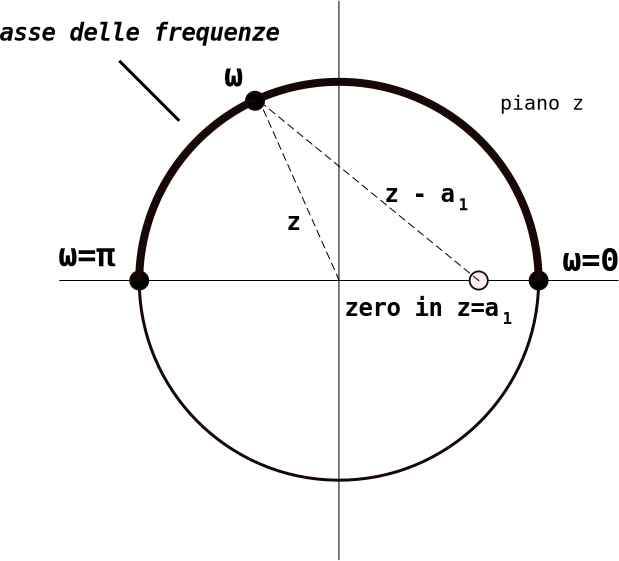
\includegraphics[width=0.4\textwidth]{\imagedir/mag_response}
				\caption{Valutazione della risposta in magnitudine per $z = e^{i
				\omega}$. Il fattore $|z - a_1|$ \`e la lunghezza del vettore dallo
				zero in $a_1$ sino al punto sul cerchio unitario corrispondente alla
				frequenza $\omega$\label{fig:mag response}}
\end{center}
\end{figure}

Ecco il significato della figura \ref{fig:mag response}: immaginiamo di
camminare sul cerchio unitario da $\omega = 0$ sino a $\omega = \pi$.
Quando ci troveremo vicino a $\omega = 0$, il modulo del vettore $|z - a_1|$
sar\`a molto piccolo e quindi influir\`aà molto sulla magnitudine del 
della funzione di trasferimento (riducendola). Man mano che ci allontaneremo
da $\omega = 0$ il modulo aumenter\`a e di conseguenza anche la magnitudine
della funzione di trasferimento. Quindi \`e ovvio che la Fig.\vref{fig:mag
response} ci sta mostrando la funzione di trasferimento di un filtro
passa--alto. Mentre per $a_1$ negativi si avrebbe un filtro passa--basso.
\begin{figure}[htp]
\begin{center}
				\includegraphics[width=0.85\textwidth]{\plotdir/zplane}
				\caption{La funzione $|\mathpzc{H}(z)|$ sul piano $z$\label{fig:mag response z plane}}
\end{center}
\end{figure}

La figura \vref{fig:mag response z plane} illustra la magnitudine della
funzione $z$ all'interno del cerchio unitario per $a_1 = 0.8$.


% completare la sezione
